\chapter{The CMS Detector}
\label{sec:cms}

The Compact Muon Solenoid (CMS) detector is one of two hermetic, general purpose detectors at the Large Hadron Collider.
The original motivation for the experiment was the discovery of the Higgs boson by observing its decays to photons, electrons, and muons.
Towards this end, the detector was built to fulfill the following goals:
\begin{itemize}
\item Unambiguous charge identification of muons with momenta up to 1\TeV
\item 1\GeV mass resolution on 100\GeV pairs of muons, electrons, and photons
\item Efficient triggering and tagging of $\tau$ lepton and $b$ quark decays
\item Good resolution on the hadronic energy and missing transverse energy
\item Sufficient time resolution to deal with 40 MHz of collisions
\end{itemize}
The CMS detector consists of four main subdetetors: the silicon pixel and strip trackers, the electromagnetic calorimeter (ECAL), the hadronic calorimeter (HCAL), and the muon chambers.
The first three are within the field volume of the eponymous 3.8 T superconducting NbTi solenoid magnet while the muon chambers are embedded in the return yoke of the magnet.
Additionally, there is an online triggering system to reduce readout from 40 MHz to $\mathcal{O}(1)$ kHz for prompt reconstruction. 

\begin{figure}[htbp]
  \centering
  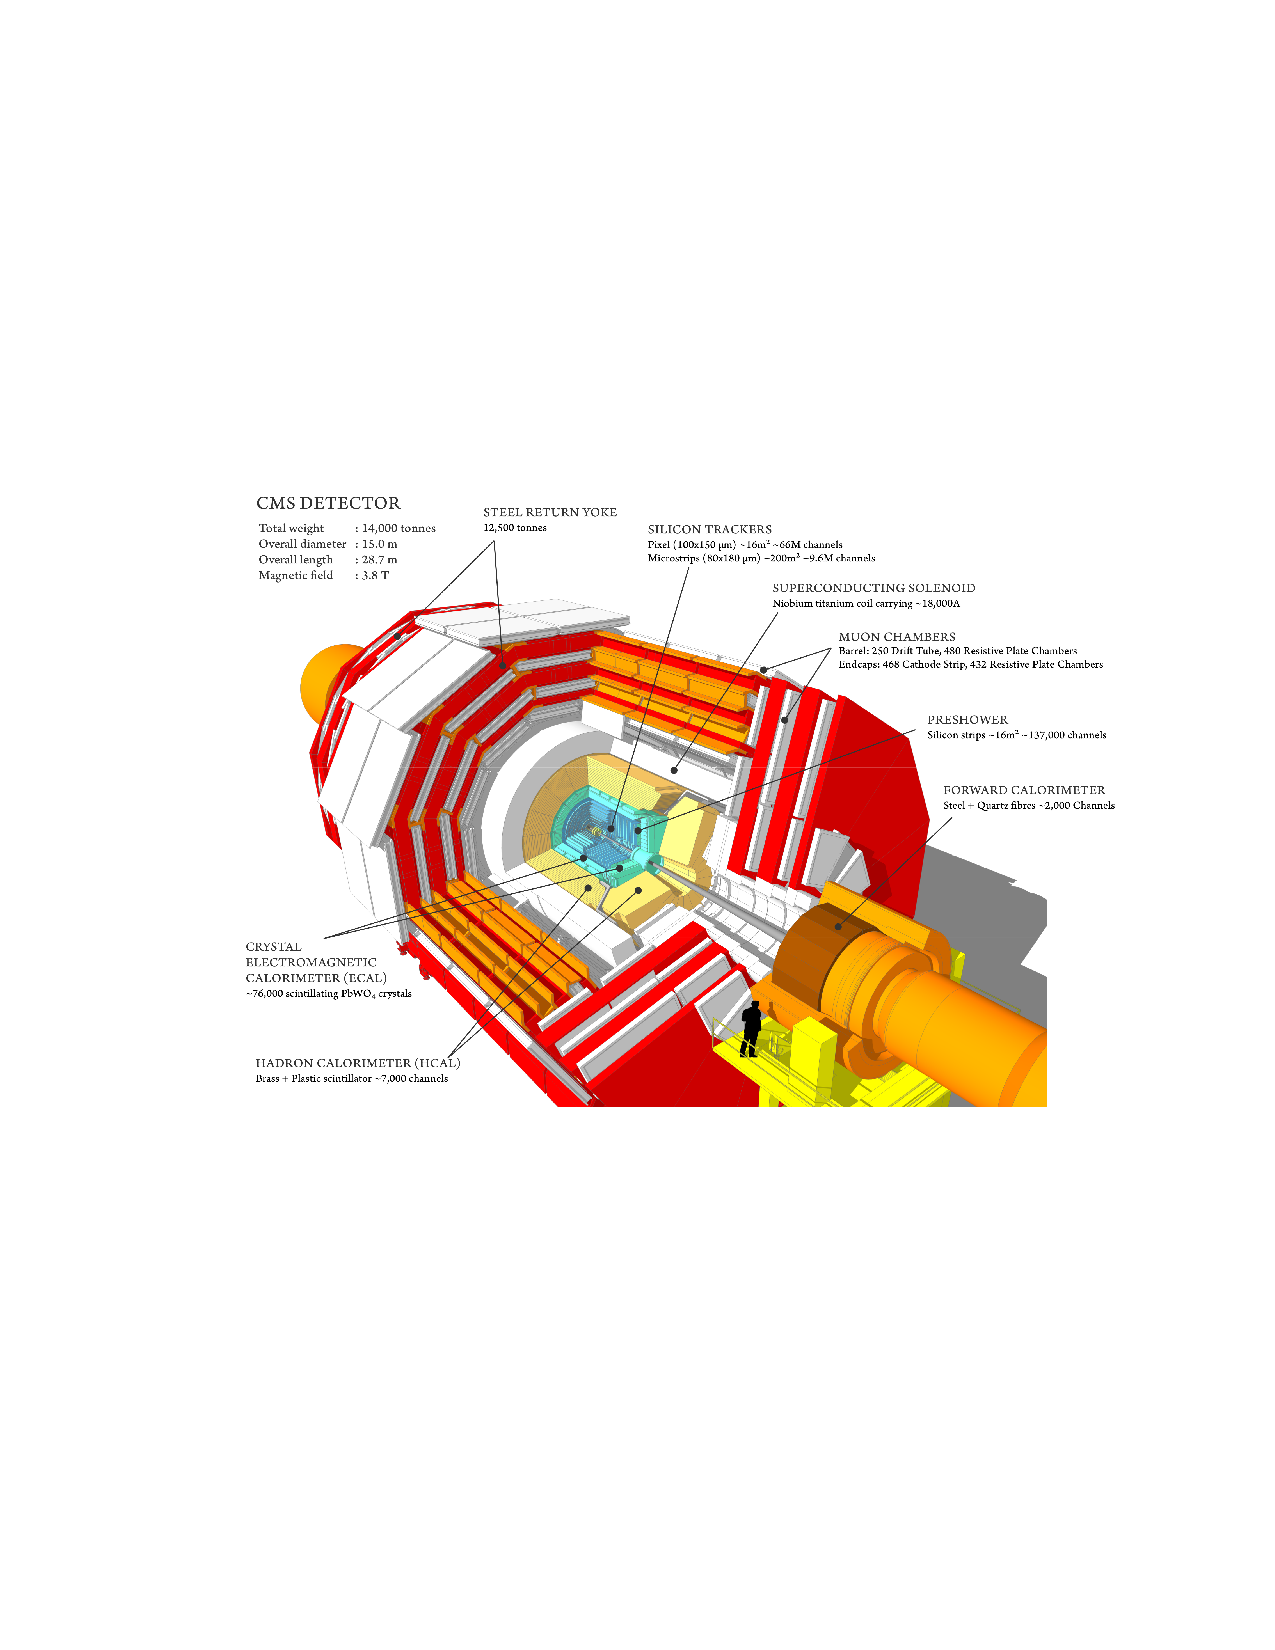
\includegraphics[width=0.9\textwidth]{Detector/Figures/cms_detector.pdf}
  \caption{
    A cutaway view of the CMS detector.
    The labels identify the solenoid as well as the different subdetectors and their components. 
    Reprinted from Reference~\cite{}. % http://cms.web.cern.ch/news/cms-detector-design
  }
  \label{fig:cms}
\end{figure}

The overall layout of the CMS detector is shown in Figure~\ref{fig:cms}. 
The CMS detector has a weight of 12500 tons, a length of 22 m, a diameter of 15 m, and a cylindrical geometry with concentric barrel shaped detectors in the central region and disc shaped detectors in the forward region.
The following coordinate system is used when working with the CMS detector:
\begin{itemize}
\item distance $z$ along the beam axis
  \begin{itemize}
  \item $z=0$ at the center of the detector
  \item positive corresponds to counter-clockwise as seen from the sky
  \end{itemize}
\item distance $r$ from the beam axis
\item polar angle $\theta$ measured with respects to the positive $z$-axis
\item azimuthal angle $\phi$ in the plane orthogonal to the beam axis
\end{itemize}
In addition to these four main coordinates, we define the right-handed cartesian $x$ and $y$ coordinates perpendicular to the beam axis, with the positive $x$-axis pointing from the center of the detector to the center of the LHC ring and the positive $y$-axis pointing upwards.

The four-momentum of a particle is $p = (p_x, p_y, p_z, E)$ in the cartesian basis 
%, where the first three components are space-like and the last one is time-like,
and a particle of mass $m$ produced at rest in the center of the detector has $p = (0, 0, 0, m)$.
While the momenta along the beam axis of the two incoming protons are equal, the momenta of the incoming partons involved in the hard scattering often are not as discussed in Section~\ref{sec:collider_pheno}.
Thus, we define two kinematic quantities that are Lorentz-invariant with respect to a boost along the beam axis:
the tranverse momentum $\ptvec = p_x \hat x + p_y \hat y$ with magnitude $\pt = \sqrt{p_x^2 + p_y^2}$ and the pseudorapidity $\eta = - \ln \tan\sfrac{\theta}{2}$.

In terms of \pt, $\eta$, and $\phi$, we have the following expressions for our cartesian variables: $p_x = \pt \cos \phi$, $p_y = \pt \sin \phi$, $p_z = \pt \sinh \eta$, and $E = \pt \cosh \eta$, with the last equality assuming the mass of the particle is negligible compared to its momentum.
In terms of our Lorentz-invariant coordinates, the four-momentum of a given particle is $p = (\pt, \eta, \phi, E)$. 
Additionally, the spatial separation of two particles is given by $\Delta R = \sqrt{(\Delta\phi)^2 + (\Delta\eta)^2}$ and the fiducial acceptance of the CMS detector is from $0 \le \phi < 2\pi$ and $-5 \le \eta \le 5$.




\section{Silicon Pixel and Strip Trackers}
\label{sec:cms_tracker}

The tiny dots and thin strips.

\section{Electromagnetic Calorimeter}

Our PbWO$_{4}$ guys.

\section{Hadronic Calorimeter}

Our big brassy boi.

\section{Muon Chambers}

The red ones.

\section{Online Trigger System}

How we choose events.

\section{Detector Simulation}

Gotta get predictions somehow.

% \section{Detector Issues}

% What went wrong.

